\label{index_md_README}%
\Hypertarget{index_md_README}%
 Drive\+POCController\+\_\+\+NXP + Drive\+POCController Software

This a Embedded-\/C based software for AC Induction Motor Controller used in the POC version of the Drive project Implementation is done here by developing the V/F Control in Embedded-\/C on the NXP microcontroller using the evaluation board\+: FRDM-\/\+KV31F. NXP Controller FRDM-\/\+KV31\+F512\+VLL12 provides us with few of the Motor Controller libraries and they are used here for realization

\DoxyHorRuler{0}


Software used \+:-\/ MCUXpresso IDE

Version of the software used \+:-\/ V-\/3.\+0

SDK Version used \+:-\/ 2.\+10.\+0

Version of the git commit \+:-\/ V-\/0.\+17.\+4

Compiler Details \+:-\/ GCC

Debugger Details \+:-\/ Open\+SDA with PEMicro Debugger

Date in which the documentation was made \+:-\/ 28th July 2022

Documentation prepared by \+:-\/ Sangeerth

People Involved in the project \+:-\/ Sreedhar Mahadevan, Sangeerth P

\href{https://www.nxp.com/design/software/development-software/mcuxpresso-software-and-tools-/mcuxpresso-integrated-development-environment-ide:MCUXpresso-IDE}{\texttt{ MCUXpresso-\/\+IDE Download Link}}

\DoxyHorRuler{0}


Software architecture V-\/1.\+5-\/ Block diagram aiding for better understanding\+:


\begin{DoxyInlineImage}
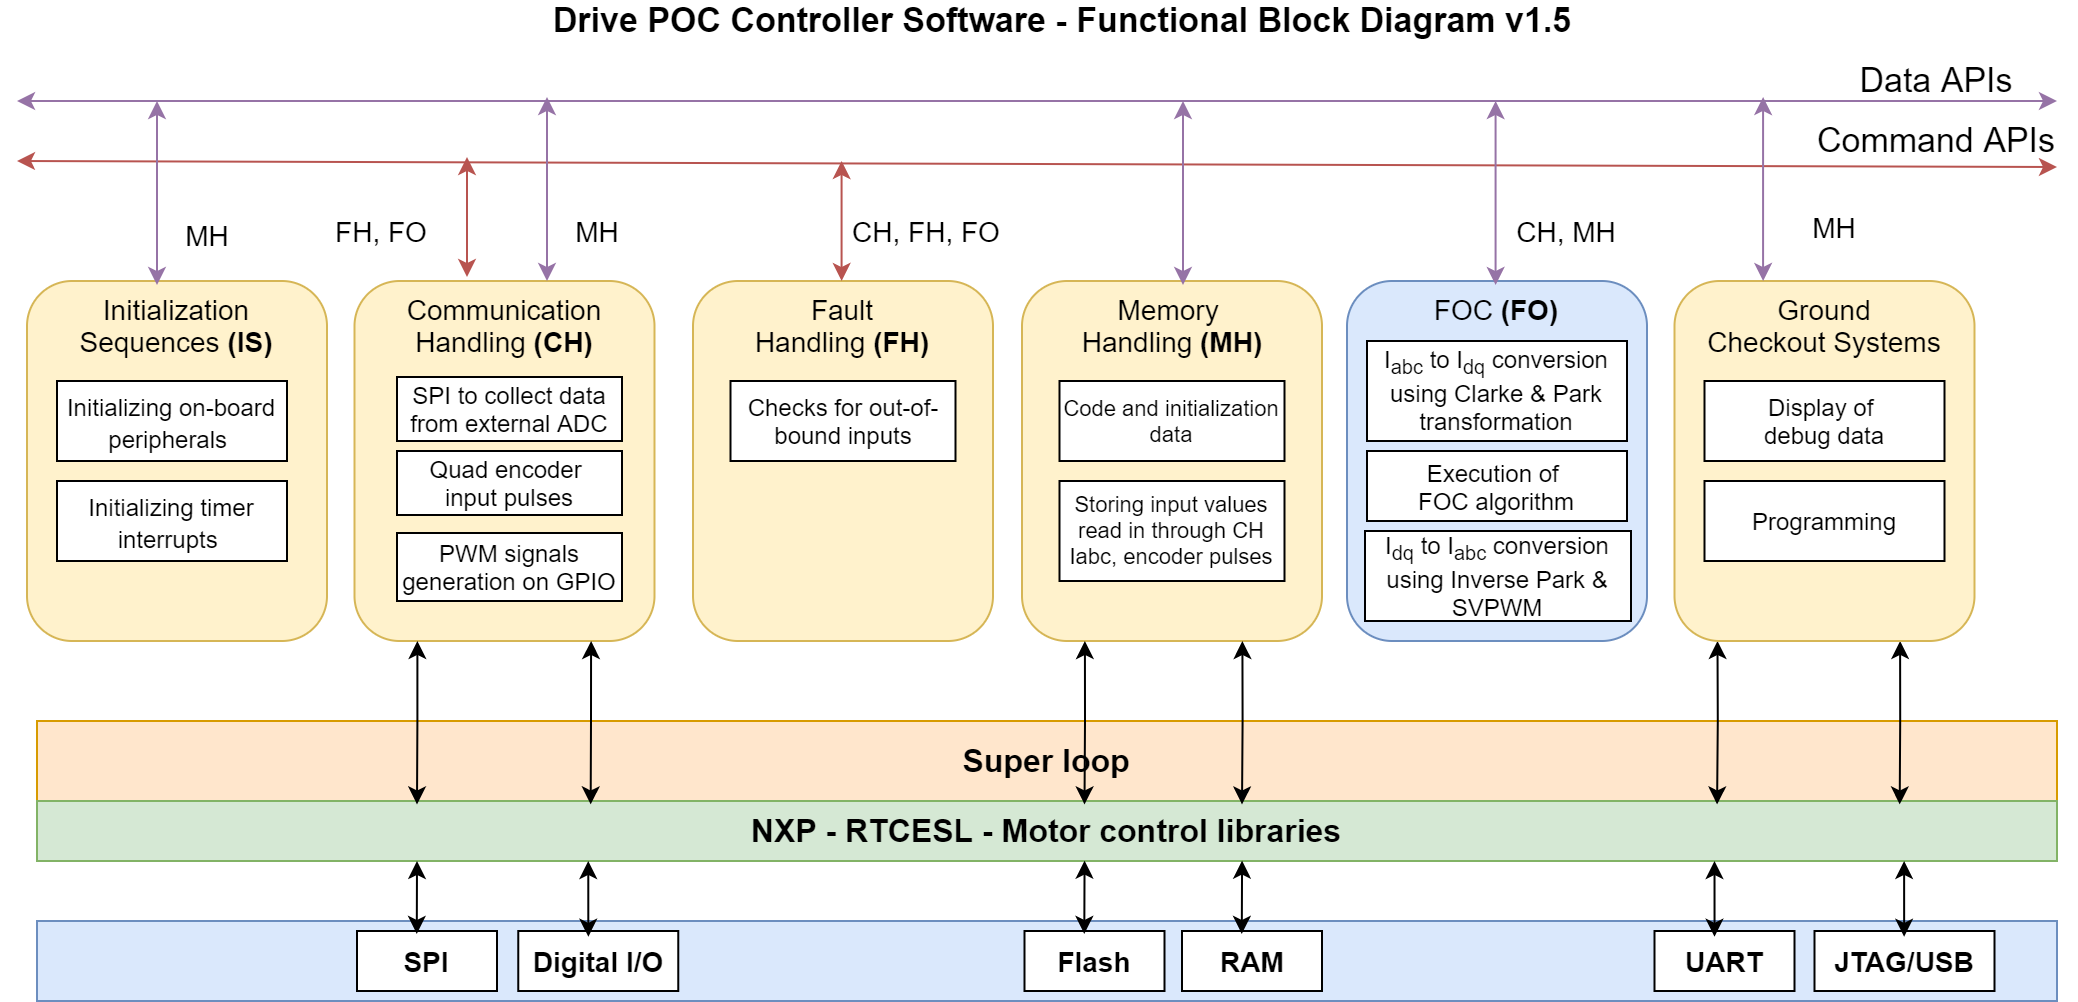
\includegraphics[height=\baselineskip,keepaspectratio=true]{software_func_block_dia.jpg}%software\+\_\+func\+\_\+block\+\_\+dia.jpg
\end{DoxyInlineImage}



\begin{DoxyImageNoCaption}
  \mbox{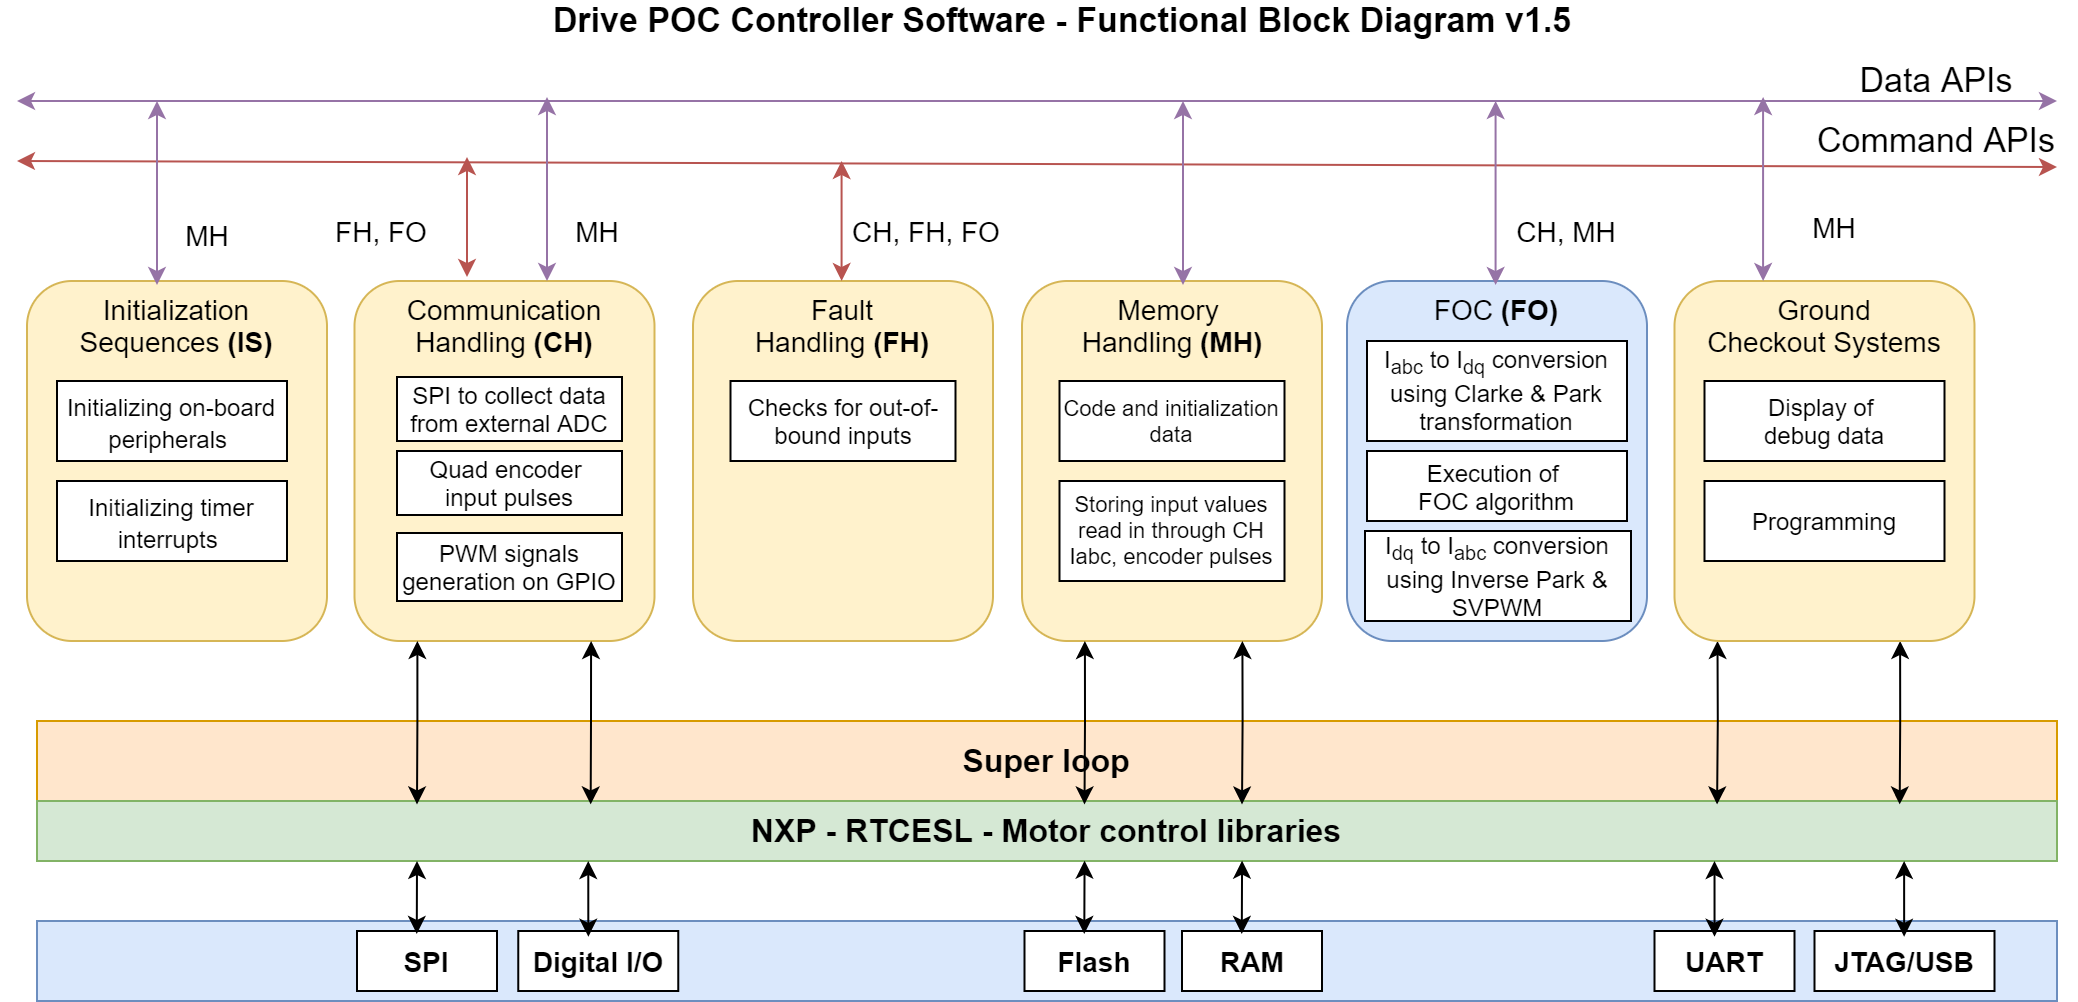
\includegraphics[width=\textwidth,height=\textheight/2,keepaspectratio=true]{software_func_block_dia.jpg}}
\end{DoxyImageNoCaption}


\DoxyHorRuler{0}


The software implementation is split across the following files\+:

The Drive\+POC\+\_\+\+Comm\+Handler has the functions that are associated with Communication of the NXP Microcontroller through its peripherals to the external world. \begin{DoxyVerb}DrivePOC_CommHandler.c && DrivePOC_CommHandler.h
\end{DoxyVerb}


The Drive\+POC\+\_\+\+Mem\+Handler has the functions that are associated with storing the values of data collected from the external world Here the MCU collects data from ADS Board to measure stator current, DC Bus current, DC Bus Voltage and stator voltages \begin{DoxyVerb}DrivePOC_MemHandler.c && DrivePOC_MemHandler.h
\end{DoxyVerb}


The Drive\+POC\+\_\+\+Control\+\_\+\+Loop has the functions associated with the V/f Algorithm Implementation for Acceleration, Steady State and Deceleration phase \begin{DoxyVerb}DrivePOC_Control_Loop.c && DrivePOC_Control_Loop.h
\end{DoxyVerb}
 The Drive\+POC\+\_\+\+Controller\+\_\+\+NXP has the main function and the PIT Interrupt functions to schedule the actions in a timed fashion \begin{DoxyVerb}DrivePOC_Controller_NXP.c && DrivePOC_Controller_NXP.h
\end{DoxyVerb}
 The Drive\+POC\+\_\+\+Fault\+Handler has the functions associated with the fault handling. For now, the fault is handled by disabling the PWM. Later on, based on ECU demands this file have to be modified. \begin{DoxyVerb}DrivePOC_FaultHandler.c && DrivePOC_FaultHandler.h 
\end{DoxyVerb}
 The Drive\+\_\+\+Parameters has the Parameters of the LOX Motor-\/\+V1.\+5.\+1, Sensor data(assumed-\/\+V1.\+0), Mosfet Data(taken from Si\+C Mosfet Datasheet) \begin{DoxyVerb}Drive_Parameters.h
\end{DoxyVerb}
 The Drive\+POC\+\_\+\+Common\+\_\+\+Header contains the structures and other datatypes that will be shared accross files. \begin{DoxyVerb}DrivePOC_Common_Header.h
\end{DoxyVerb}


\DoxyHorRuler{0}
 